
\section{Susceptibility calculations}
    \label{Sec:ResD:SubsceptibilityCalculation}

To verify that we do get enhanced susceptibility, leading to a spin-density wave state, the $q$-dependant susceptibility -- described in section \ref{Sec:1:NestingSusceptibility} -- was calculated. Since the Lindhard function takes the sum over all energies in the Brillouin zone, there may be some concern that the rather crude adjustments to the DFT calculations performed in the previous section -- which have only been verified to be correct for energies at the Fermi surface -- may give erroneous results. However the nature of the Lindhard function means that far greater weight is given to energies that are near the Fermi surface and so, assuming that the energy dispersion does vary smoothly close to the Fermi level, any differences away from the Fermi level should not be a cause for concern.  
\begin{figure}[htbp]
    \begin{center}
        \includegraphics[scale=0.9]{Chapter-dHvABaFe2P2/Figures/AngleDepMeasurements/ShiftedBandStructure/ShiftedBandStructure}
        \caption{Band structure for the bands that cross the fermi surface shifted to fit the dHvA data. (a) and (b) give an idea of the granularity of the \WIEN calculation at the Fermi surface. Inset shows the path around the brillouin zone.}
        \label{Fig:ResD:ShiftedBandStructure}
    \end{center}
\end{figure}
Calculations were performed using the \code{calc_x0.m} code described in section\ref{Sec:Exp:Susceptibility} using a $93\times93\times93$ grid of energy values that covered the first Brillouin zone. We will need to smooth over the granularity of the \WIEN band model since for the imaginary part at least, the calculations is very sensitive to slight imperfections in cancellation. Figure~\ref{Fig:ResD:ShiftedBandStructure} shows the band structure shifted as described in the previous section. We notice that away from the Fermi surface we have dicontinuities in the large hole pocket, most notably between $Z$ and $\Sigma_1$, due to the correction applied which is proprtional to the \DzTwo character however these are reasonably far from the Fermi level. Two regions in the figure are marked (a) and (b) which show points around the Fermi level as they are spaced in the $93\times93\times93$ model. (a) is particularly steep and has a $\Delta \epsilon/\textrm{pt.} = \unit[0.0760]{Ry}$ and (b) is more typical of the gradient at the Fermi level and has $\Delta \epsilon/\textrm{pt.} = \unit[0.0368]{Ry}$. So the energy scale that will need to compensated is \unit[$\sim 5\times10^{-2}$]{Ry}.



A small $\delta$ of $10^{-6}$ was included in order to obtain the imaginary component of the susceptbility.

\begin{figure}[htbp]
    \begin{center}
        \includegraphics[scale=0.9]{Chapter-dHvABaFe2P2/Figures/Susceptibility/2DSusceptibility/2DSusceptibility}
        \caption{Left panel shows the maximum $q$ dependant susceptibility in each plane perpendicular to $q_z$ between bands $1$ and $4$. Results where calculated with \unit[1]{mRy} of temperature smearing and $\delta=1\times10^{-6}$. Right panel shows the susceptibility in the plane at $q_z=1.5$ which is typical of all the $q_z$ planes for this band combination.}
        \label{Fig:ResD:SusceptbilityEnhancement}
    \end{center}
\end{figure}

\Fig\ref{Fig:ResD:FullSusceptibility} shows the total susceptibility coupling across various band combinations.

\begin{figure}[htbp]
    \begin{center}
        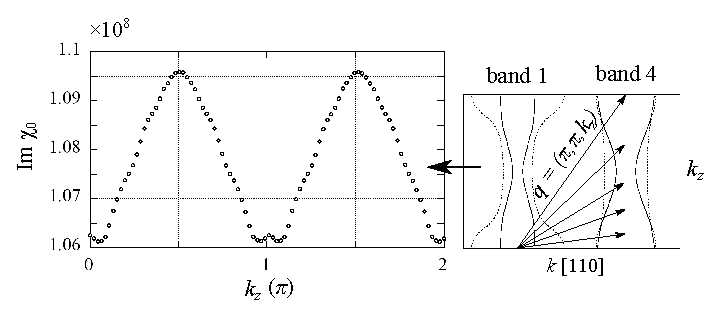
\includegraphics[scale=0.9]{Chapter-dHvABaFe2P2/Figures/Susceptibility/NestingVector/NestingVector}
        \caption{}
        \label{Fig:ResD:FullSusceptibility}
    \end{center}
\end{figure}

